\documentclass[12pt]{article}
\usepackage{amssymb}
\usepackage{amsmath}
\usepackage{amsfonts}
\usepackage{graphicx}
\usepackage{float}
\usepackage{forloop}
\usepackage{tikz}
\usepackage[bottom=1in,top=1in,left=1in,right=1in]{geometry}

\begin{document}

{\bf Keywords:} Intrinsic variables, partial observations, complex dynamical systems

\section{Introduction}

\begin{itemize}
    \item We know that manifold learning can lead to reduction in reducible complex dynamical systems

    \item We know from recent Ronen that if we do IV we can ``merge'' data sets

    \item We know from recent Neta that LapPyr (especially with new adaptive twists) can be used to interpolate function on sampled data and, in, particular, or reduced representations of sample data

    \item Here, we synthesize these three ideas to show that if we have partial measurements for ``complex but effectively low-dimensional'' systems, we can reconstruct/estimate the missing measurements based on a training set.

    \item This is important in both open loop sensing and in closed control loops based on the measurements of unavailable variables

    \item Two examples that arise in typical physicochemical computations, one from chemical reactions and one from MD

    \item Both examples are NOT SDEs but it is established/accepted that they can be effectively modeled as SDEs.

    \item Sometimes we can predict variables and sometimes we can predict statistics of variables --- maybe best to bring it up WITHIN the examples
\end{itemize}

\section{Methods}

\subsection{Intrinsic Modeling}
\begin{figure}[H]
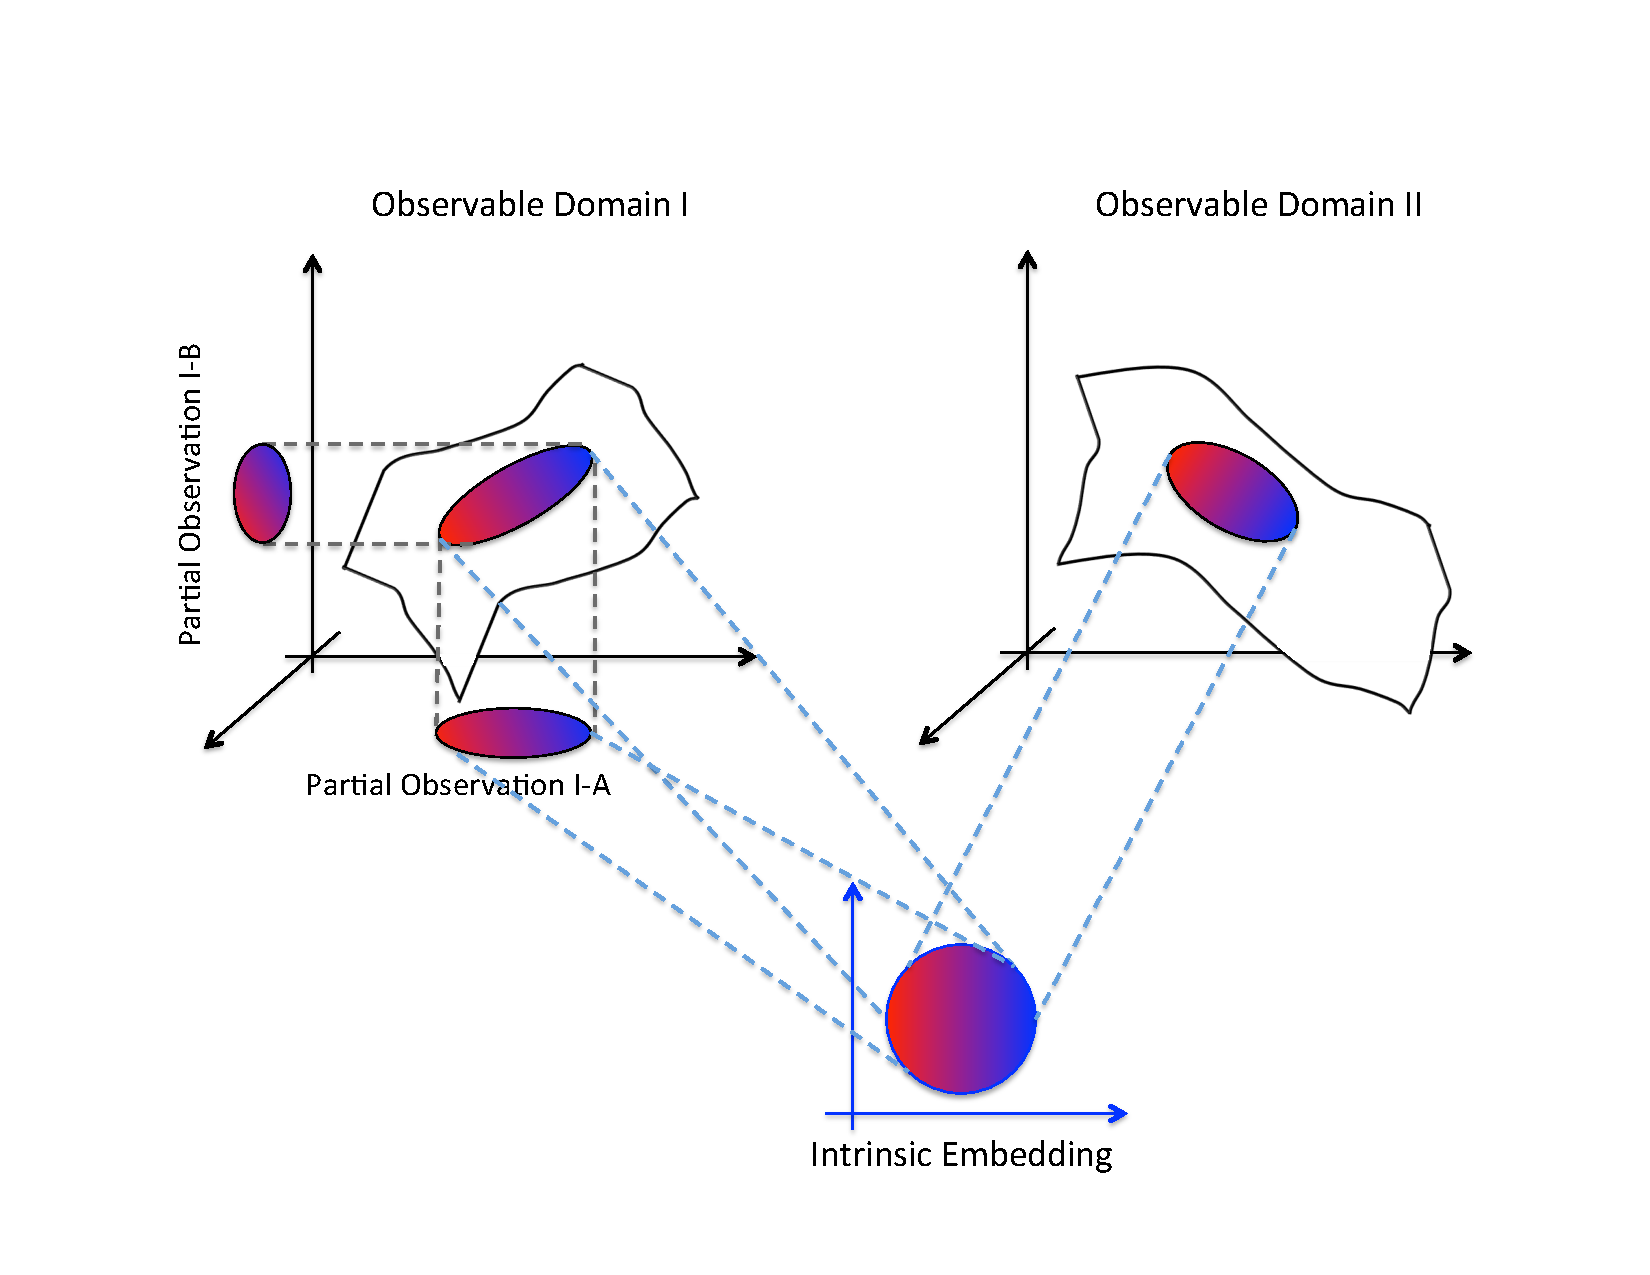
\includegraphics[width=\textwidth]{IntrinsicEmbeddingIllustration2.pdf}
\caption{Illustration of the nonlinear embedding that yields an intrinsic representation independent of measurement modality. (Left) The underlying variables in which the diffusion parameters are independent with unit variance. The depicted points illustrate the end points of the short bursts that create a sphere around the initial point on the manifold. (Right Top) The first set of observed variables. The depicted points illustrate the end points of the short bursts as observed via the first observation modality. (Right Bottom) The second set of observed variables. The depicted points illustrate the end points of the short bursts as observed via the second observation modality.}
\end{figure}

{\bf To do:} \\
Block diagram/algorithm

\subsection{Laplacian Pyramids}

{\bf To do:} \\
A flow chart/block diagram of the method (possibly with the formulas).\\
Maybe an illustration of the multiscale reconstruction of functions.

\begin{figure}[H]
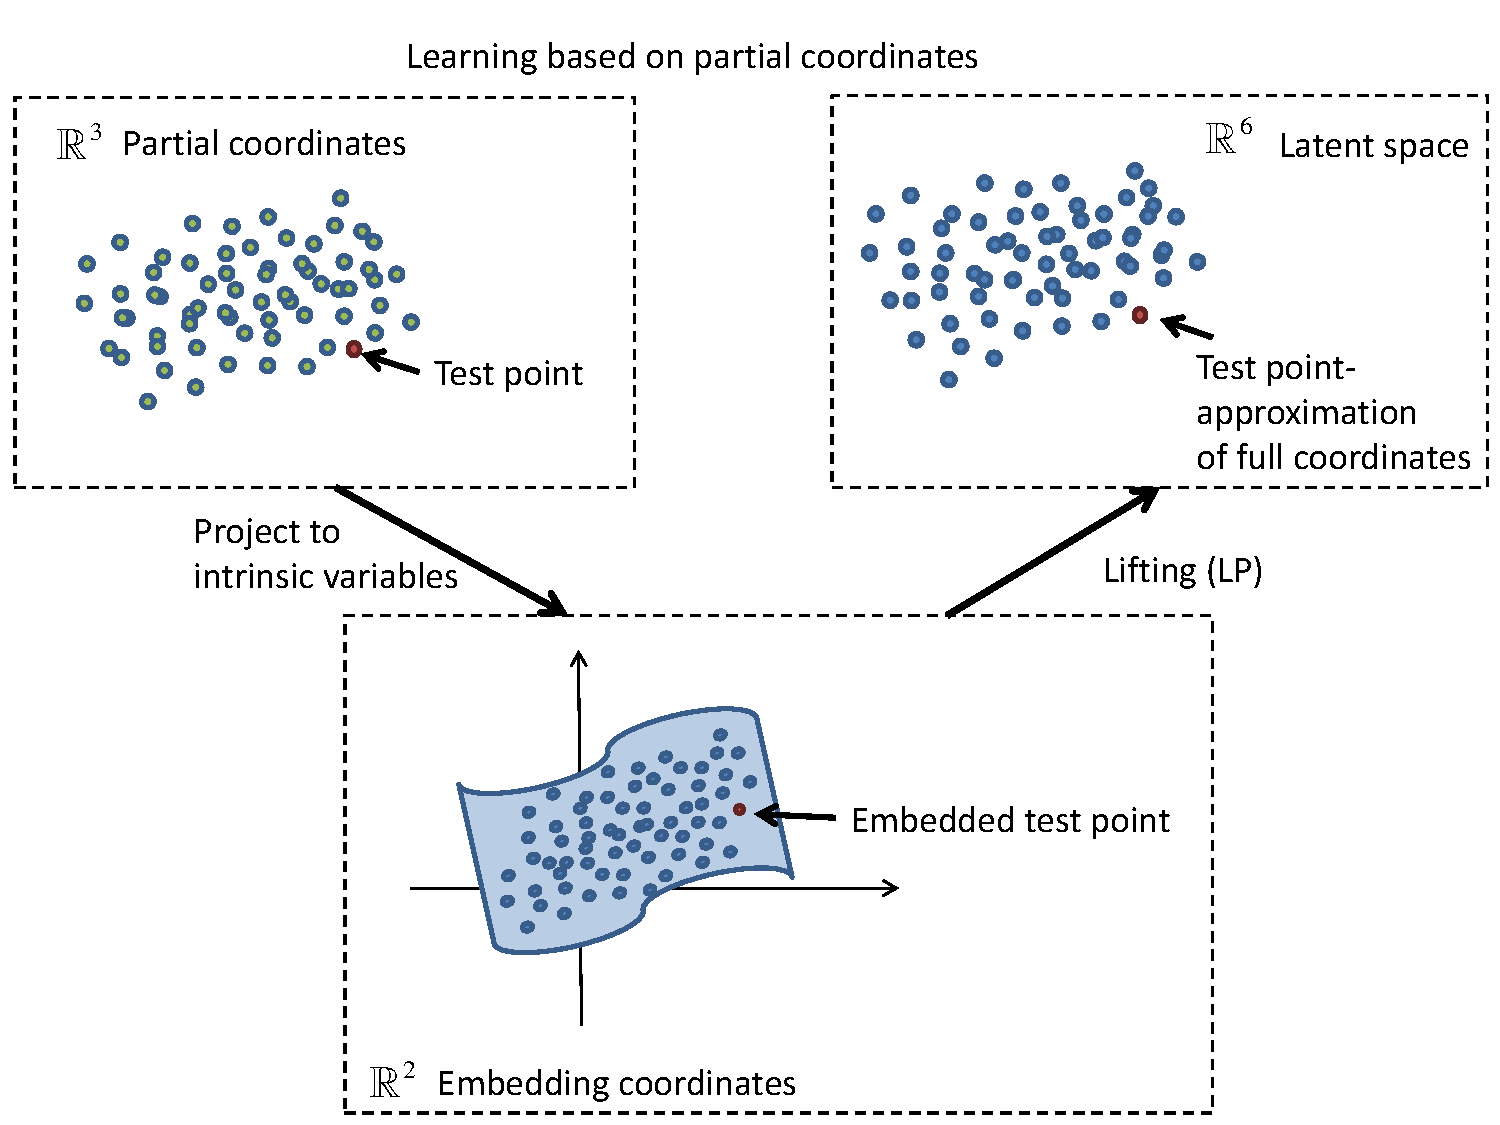
\includegraphics[width=\textwidth]{LapPyr_illustration.pdf}
\caption{Illustration of overall methodology}
\end{figure}

\section{Models and Results}

\subsection{Chemical Reaction Network}

\begin{figure}[H]
  \includegraphics[height=6cm]{rxn_figures/rxn_manifold1.jpg}\llap{\raisebox{3.5cm}{\includegraphics[height=2.5cm]{rxn_figures/rxn_manifold1_2.jpg}}}
  \includegraphics[height=6cm]{rxn_figures/rxn_manifold2.jpg}\llap{\raisebox{3.5cm}{\includegraphics[height=2.5cm]{rxn_figures/rxn_manifold2_2.jpg}}} \\
  \includegraphics[height=6cm]{rxn_figures/rxn_manifold3.jpg}\llap{\raisebox{3.5cm}{\includegraphics[height=2.5cm]{rxn_figures/rxn_manifold3_2.jpg}}}
  \includegraphics[height=6cm]{rxn_figures/rxn_manifold4.jpg}\llap{\raisebox{3.5cm}{\includegraphics[height=2.5cm]{rxn_figures/rxn_manifold4_2.jpg}}} \\
%    \includegraphics[width=0.5\textwidth]{rxn_figures/rxn_manifold1.jpg}
%    \includegraphics[width=0.5\textwidth]{rxn_figures/rxn_manifold2.jpg}\\
%    \includegraphics[width=0.5\textwidth]{rxn_figures/rxn_manifold3.jpg}
%    \includegraphics[width=0.5\textwidth]{rxn_figures/rxn_manifold4.jpg}
    \caption{Projections of manifold onto different chemical components. The insets show a different projection to illustrate the two-dimensionality of the manifold.}
\end{figure}

\begin{figure}[H]
    \includegraphics[width=0.5\textwidth]{rxn_figures/rxn_NLICA1.jpg}
    \includegraphics[width=0.5\textwidth]{rxn_figures/rxn_NLICA2.jpg}
    \includegraphics[width=0.5\textwidth]{rxn_figures/rxn_NLICA_corr1.jpg}
    \includegraphics[width=0.5\textwidth]{rxn_figures/rxn_NLICA_corr2.jpg}
    \caption{(Top) IV embedding obtained from observations of components 1, 2, 4, and 6 (left) embedding obtained from observations of components 1, 2, 3, and 5 (right), colored by component 1 (left) (Bottom) Correlation of first IV (left, correlation=0.97) and second IV (right, correlation=0.95) between two different embeddings.}
\end{figure}

\begin{figure}[H]
    \includegraphics[width=0.5\textwidth]{rxn_figures/chm4_from_Em.png}
    \includegraphics[width=0.5\textwidth]{rxn_figures/chm6_from_Em.png}
    \caption{Laplacian Pyramids (LapPyr) and nearest neighbor (nn) reconstructions of species 4 (left) and 6 (right). The nearest neighbors are computed both in the embedded space and in the ambient space, and in the embedded space.}
\end{figure}

The nearest neighbor reconstruction using neighbors in the ambient space is more accurate than the other two methods, implying that some of the error arises from inaccuracies in the embeddings.
%
However, we would like to note that computing nearest neighbors in the ambient space requires knowing how to map full observations to partial observations.
%
Therefore, in cases where we have partial {\em unknown} observations (i.e. we observe some chemicals, but we do not know which ones), we can still use the embedded space (intrinsic variables) to predict the remaining species.

\subsection{Alanine Dipeptide}

\begin{itemize}
  \item 10000 data points
  \item The NLICA embeddings were computed using odd and even atoms (atoms 1 and 3 were removed)
  \item Laplacian Pyramids were then used to predict the atom positions for the test data using the IV representation
\end{itemize}

\begin{figure}[H]
    \includegraphics[width=0.6\textwidth]{FES.pdf}
    \includegraphics[width=0.4\textwidth]{molecule_labeled2.jpg}
    \caption{(Left) Free energy surface for Alanine Dipeptide. The minima are labeled A, B, and C, and the corresponding molecular configurations are shown. (Right) The molecular structure of Alanine Dipeptide. The atoms are numbered and the two dihedral angles $\phi$ and $\psi$ are indicated.}
\end{figure}

The motion of Ala2 can be well described by three IV.
%
The first IV describes the flipping of the first and third atoms, the second IV describes the dihedral angle $\phi$, and the third IV describes the dihedral angle $\psi$.

\begin{figure}[H]
    \includegraphics[width=0.5\textwidth]{ala_figures_evenodd/NLICA_corr.jpg}
    \includegraphics[width=0.5\textwidth]{ala_figures_evenodd/DM_corr.jpg}
    \caption{(Left) Correlation between the second IV computed using the odd atoms and the even atoms. (Right) Correlation between the second DM computed using the odd atoms and the even atoms.}
\end{figure}

\begin{table}
\begin{tabular}{| r || c | c |}
  \hline
  & Coordinate 1 & Coordinate 2 \\
  \hline
  \hline
  NLICA & 0.62 & 0.84 \\
  \hline
  DM & 0.54 & 0.60 \\
  \hline
\end{tabular}
\caption{Correlation between the embedding coordates from NLICA and DMAPS using the odd and even atoms.}
\end{table}

\begin{table}
\begin{tabular}{| r || c | c | c |}
  \hline
  & Coordinate 1 & Coordinate 2 & Coordinate 3 \\
  \hline
  \hline
  NLICA & 0.97 & 0.72 & 0.85 \\
  \hline
  DM & 0.95 & 0.76 & 0.74 \\
  \hline
\end{tabular}
\caption{Correlation between the embedding coordinates from NLICA and DMAPS using all and just odd coordinates.}
\end{table}


\begin{figure}[H]
    \includegraphics[width=0.3\textwidth]{ala_figures_allodd/ala2_embed1.jpg}
    \includegraphics[width=0.3\textwidth]{ala_figures_allodd/ala2_embed2.jpg}
    \includegraphics[width=0.3\textwidth]{ala_figures_allodd/ala2_embed3.jpg}
    \caption{The 3-dimensional embedding for Alanine Dipeptide using all the atoms, colored by the y-coordinate of the first atom (left), the dihedral angle $\phi$ (center), and the dihedral angle $\psi$ (right).}
\end{figure}


\begin{figure}[H]
  \centering
%  \newcounter{atomnumber}
%  \forloop{atomnumber}{1}{\value{atomnumber} < 11}{
%    \includegraphics[width=0.15\textwidth]{ala_figures_allodd/ala2_recon_corr_\arabic{atomnumber}_1.jpg}
%    \includegraphics[width=0.15\textwidth]{ala_figures_allodd/ala2_recon_corr_\arabic{atomnumber}_2.jpg}
%    \includegraphics[width=0.15\textwidth]{ala_figures_allodd/ala2_recon_corr_\arabic{atomnumber}_3.jpg}\\
%  }
    \foreach \atomnumber in {1,2,3,6,8} {
        \includegraphics[width=0.2\textwidth]{ala_figures_allodd/ala2_recon_corr_\atomnumber_1.jpg}
        \includegraphics[width=0.2\textwidth]{ala_figures_allodd/ala2_recon_corr_\atomnumber_2.jpg}
        \includegraphics[width=0.2\textwidth]{ala_figures_allodd/ala2_recon_corr_\atomnumber_3.jpg}\\
      }
  \caption{The correlation between the true position and the reconstructed position for atoms 1, 2, 3, 6, and 8 (using Laplacian Pyramids) for each coordinate for the NLICA embedding of the odd data, using the NLICA embedding from all coordinates as training data.}
\end{figure}

\begin{figure}[H]
    \includegraphics[width=0.3\textwidth,trim=0.5in 3in 4in 0.5in, clip]{molec_figures/molecule300.jpg}
    \includegraphics[width=0.3\textwidth,trim=0.5in 3in 4in 0.5in, clip]{molec_figures/molecule600.jpg}
    \includegraphics[width=0.3\textwidth,trim=0.5in 3in 4in 0.5in, clip]{molec_figures/molecule900.jpg}    
    \caption{True structure (black) and reconstructed structure (red) for three different data points}
\end{figure}

\section{Conclusions}

\end{document}
